%%%%%%%%%%%%%
%  Ch1 : Introduction  %
%%%%%%%%%%%%%

\chapter{Introduction}
Before beginning the summary, I want to tell you that my English level isn't perfect. Please collaborate and correct the grammatically wrong sentences.\\

\section{Reminder}
The governing equations in transport processes are the followings :
\begin{itemize}
	\item[$\bullet$] Mass conservation : 
	      \begin{equation}
	      	\frac{\partial \rho}{\partial t} + \nabla (\rho v) = 0
	      \end{equation}
	\item[$\bullet$] Navier-Stokes :
	      \begin{equation}
	      	\rho \left(\frac{Dv}{Dt} + v \nabla v \right) = -\nabla p + \mu \nabla ^2 v
	      \end{equation}		 
	\item[$\bullet$] Energy equation :
	      \begin{equation}
	      	\frac{DT}{Dt} = \nabla (\alpha \nabla T) + \frac{\dot{Q}v}{\rho c}
	      \end{equation}
	\item[$\bullet$] Species conservation
	      \begin{equation}
	      	\frac{\partial \rho _A}{\partial t} + \nabla (\rho _A v_A) = r_A
	      \end{equation}
\end{itemize}
Let's specify that there are many applications using these equations like in the aerospace and automotive industry, in safety and fire prevention or in buildings design.  
	
\section{Convection and diffusion}
\subsection{Definitions}
\begin{wrapfigure}[8]{l}{6cm}
	\vspace{-5mm}
	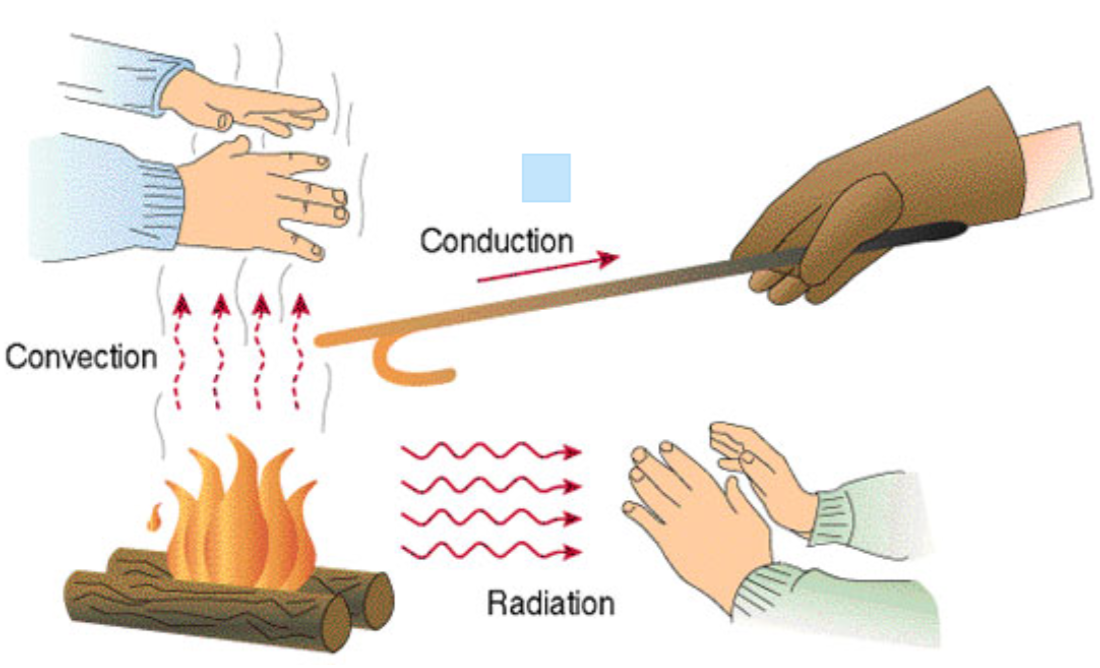
\includegraphics[scale=0.3]{ch1/1}
\end{wrapfigure}
Here is a picture illustrating the principles of \textbf{convection}, \textbf{conduction} and \textbf{radiation}. Imagine that you have a fire and you put your hands above. You will feel a flow of heat transmitted by convection. If someone comes with a stick, there will be conduction in the material transmitting the energy from particles to particles. Finally, if the hands are next to the fire, there is no flow but you feel the heat. The energy is transmitted by radiation. 
	
\newpage

\subsection{Convection}
\begin{wrapfigure}[4]{r}{3.5cm}
	\vspace{-5mm}
	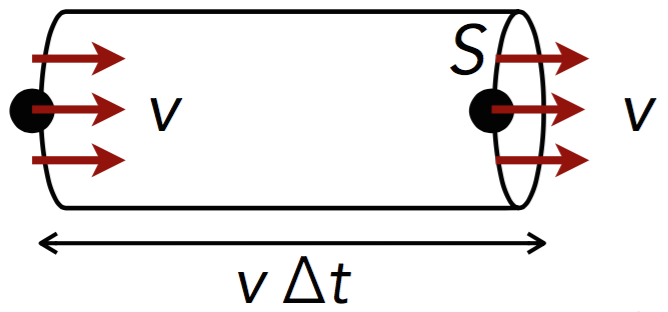
\includegraphics[scale=0.3]{ch1/2}
\end{wrapfigure}
Convection is a transfer always associated to \textbf{bulk (ensemble) fluid motion}. We consider a fluid with \textbf{uniform} velocity and a cylinder of section S and length $v \Delta t$. In that time interval, the fluid in the cylinder will have crossed the section S. We are now able to express the convective flux of momentum (quantité de mouvement), energy and mass knowing that the flux of a physical quantity is given by 
\begin{equation}
	\text{flux}_A = \frac{A}{S\Delta t}
	\label{equation:1.5}
\end{equation}
	
\subsubsection{Mass}
We know that the mass is given by density $\times$ volume and that the volume of the cylinder is $Sv\Delta t$. Using the new expression of the mass and \eqref{equation:1.5}, we can find the \textbf{flux of mass} 
\begin{equation}
	M_c = \rho v S \Delta t \qquad and \qquad  J_{M_c} = \frac{M_c}{S\Delta t} = \rho v
\end{equation}
	
\subsubsection{Momentum}
Similarly to the calculus of the mass
\begin{equation}
	Q_c = mv = \rho v^2 S \Delta t \qquad and \qquad J_{Q_c} = \rho v^2
\end{equation}
	
\subsubsection{Energy}
The energy in the system is given by the specific heat energy of each particles\footnote{See \emph{Chimie générale} for the expression}. If $T_0$ is the reference temperature, 
\begin{equation}
	E_c = \rho c_v v (T-T_0) S \Delta t \qquad and \qquad J_{E_c} = \rho c_v v (T-T_0)
\end{equation}
	
\subsection{Diffusion}
\begin{wrapfigure}[4]{l}{3.5cm}
	\vspace{-5mm}
	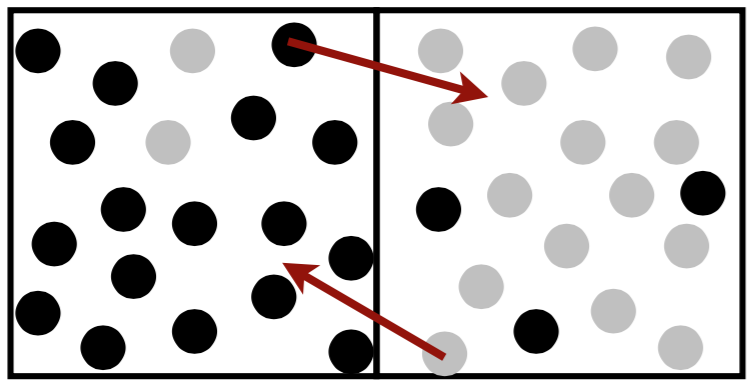
\includegraphics[scale=0.26]{ch1/3}
\end{wrapfigure}
Diffusion is a transfer associated to the \textbf{particles	random walk} and is due to the presence of a gradient of physical quantity (temperature for example). The picture on the left illustrates that, for an infinite time, the process will reequilibrate the gradient, difference between the two boxes.
	
\section{Diffusive flux}
\begin{wrapfigure}[3]{r}{5.5cm}
	\vspace{-5mm}
	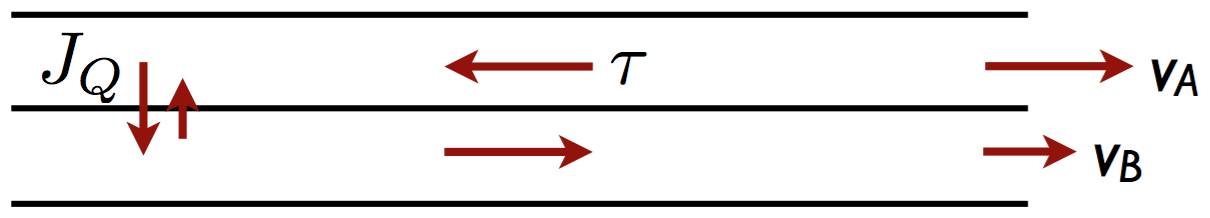
\includegraphics[scale=0.26]{ch1/4}
\end{wrapfigure}
If we consider two parallel fluid layers to bulk velocity $v_A > v_b$, the gradient of velocity will vanish\footnote{Disparaître} ($v_A = v_b$). This effect is due to the initial velocity gradient that cause the diffusion of faster particles towards the slower ones, transferring a momentum flux $J_Q$. In fact, the origin of the flux in the transversal direction to the flow is due to the \textbf{friction} between the two layers, parallel to the flow direction. 
	
\subsection{Shear stress}
To characterize the friction between to layers, we introduce the \textbf{shear stress}\footnote{Contrainte de cisaillement} that is proportional to the gradient of velocity
\begin{equation}
	\tau = \tau \left( \frac{dv}{dy} \right)
\end{equation}
According to the Newton's law, for Newtonian fluids like gases and liquids, the equation becomes
\begin{equation}
	\tau = \mu \left( \frac{dv}{dy} \right)
\end{equation}
\begin{wrapfigure}[9]{l}{4cm}
	%	\vspace{-5mm}
	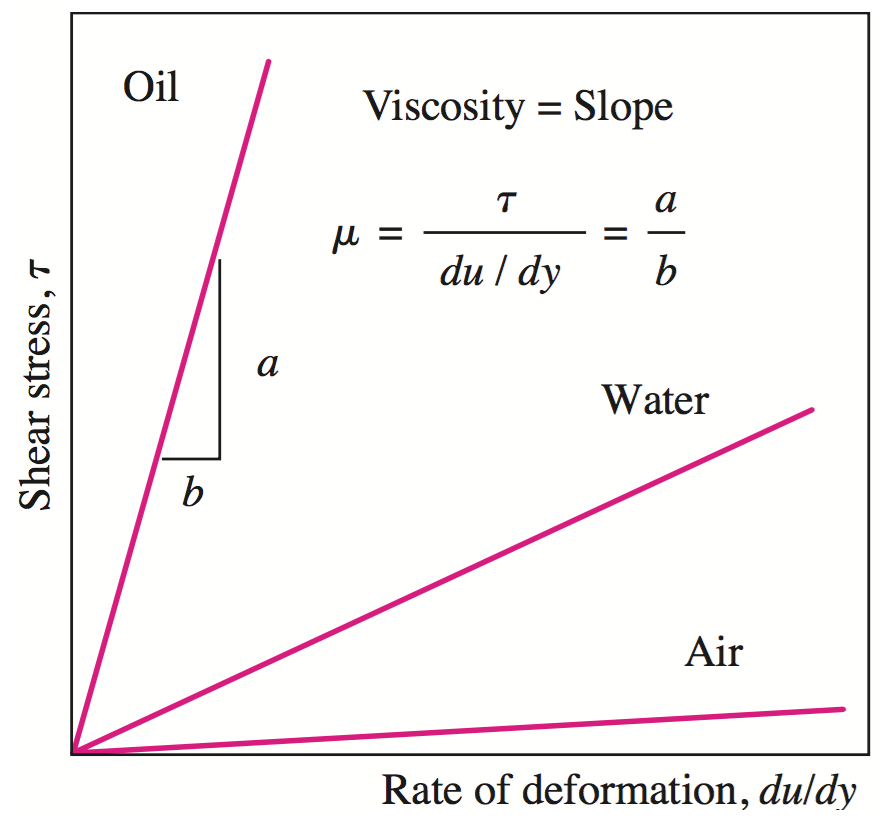
\includegraphics[scale=0.26]{ch1/5}
\end{wrapfigure}
\begin{itemize}
	\item $\mu$ is the \textbf{dynamic viscosity}, the \textbf{intrinsic resistance} of the fluid to motion $[kg/m.s]$
	\item $dv/dy$ the gradient of velocity $[s^{-1}]$
	\item $\tau$ a force per unit surface $[N/m^2] = [Pa]$
\end{itemize}
\ \\
If we see the shear stress to the \textbf{rate of deformation} \footnote{Gradient of velocity} on a graph, we can see that the \textbf{viscosity} is the slope\footnote{La pente}. We can also see that viscosity of air is miner than water that's miner than oil. 
	
\subsection{Planar Couette flow}
\begin{wrapfigure}[5]{r}{5.5cm}
	\vspace{-5mm}
	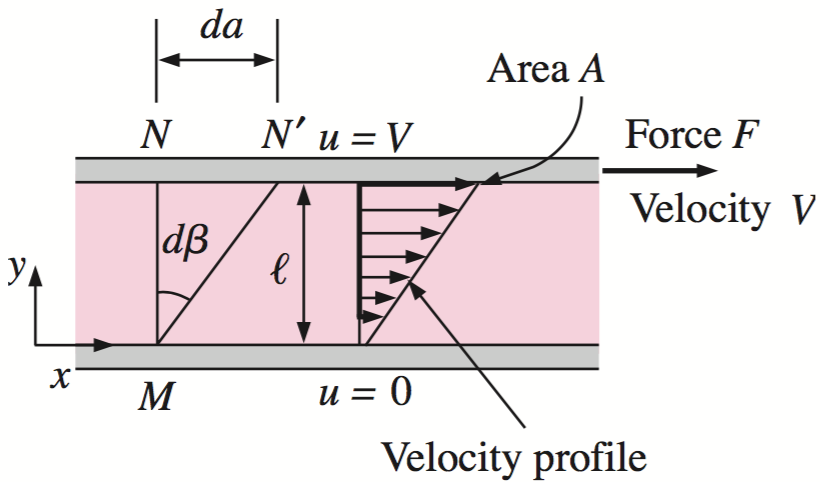
\includegraphics[scale=0.4]{ch1/6}
\end{wrapfigure}
Let's consider a fluid layer between two very large plates separated by a distance $l$. A constant parallel force $F$ (drag force\footnote{Force de traînée}) is applied to the upper plate and after the initial transients, it moves continuously to a constant velocity $V$. What are the consequences on the fluid ? \\
	
\begin{itemize}
	\item[•] \textbf{Empirical observations : }\\
	      No slip conditions\footnote{Condition de non-glissement} at walls $\rightarrow u(0) = 0$ and $u(l) = V$. \\
	\item[•] \textbf{The flow is organized in parallel layers :}\\
	      We suppose that the flow is laminar (no turbulence), so the velocity profile is a sole function of y and is \textbf{linear} : $u(y) = V\frac{y}{l}$.\\
	\item[•] \textbf{The drag force is imposed :} \\
	      $\tau = \frac{F}{A} = \mu \frac{dv}{dy} = c$
\end{itemize}
	
\newpage
	
\subsection{Fluid rheology}
\begin{wrapfigure}[12]{l}{8.5cm}
	\vspace{-5mm}
	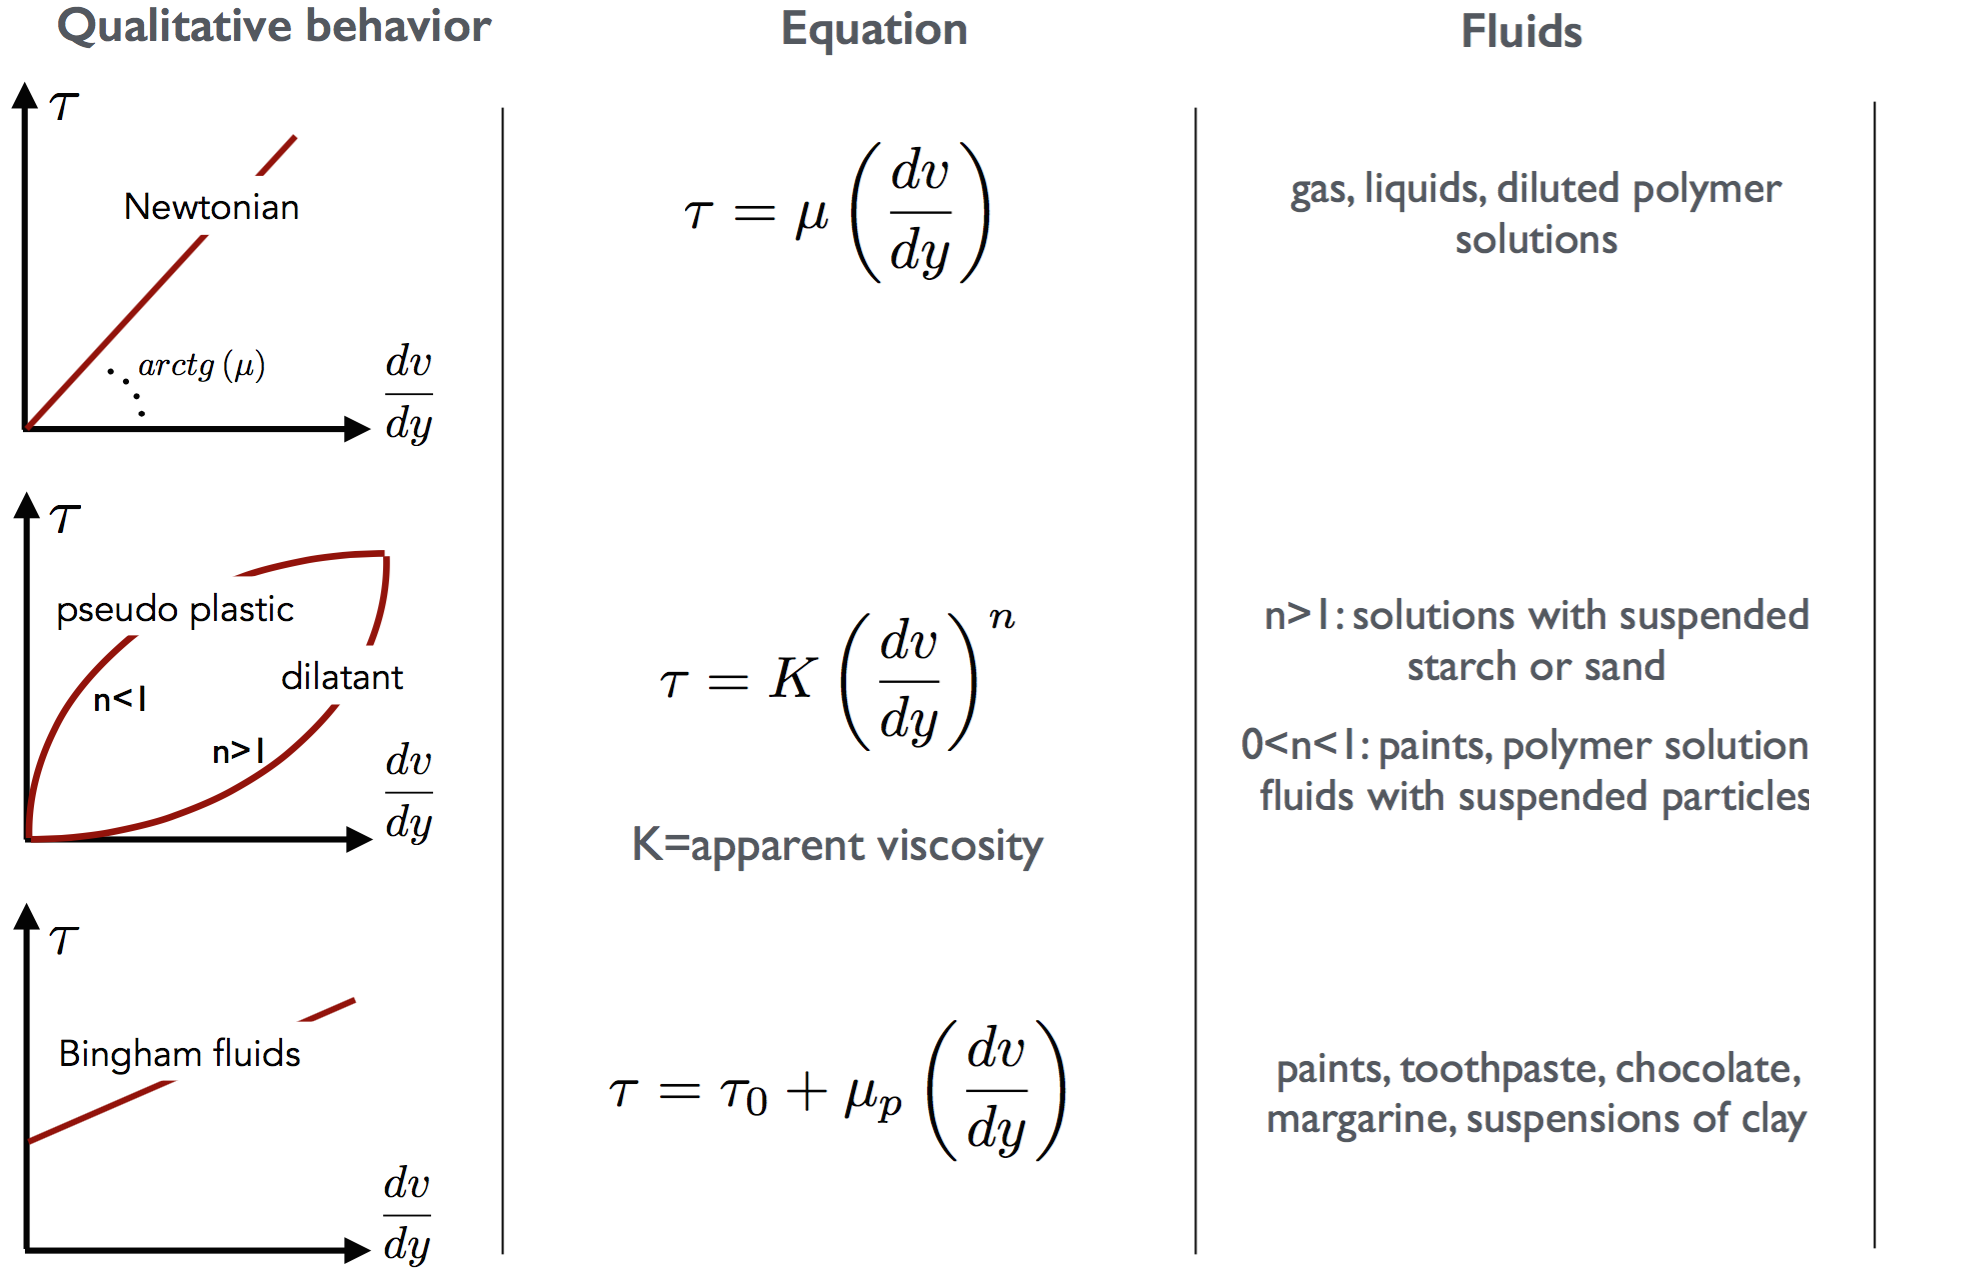
\includegraphics[scale=0.25]{ch1/7}
\end{wrapfigure}
\textbf{Rheology} is the study of the flow that establish the relation between the shear stress and the velocity gradient. Let's have a look to different fluids. \\
As first observation, we can see that Newtonian fluids respect a linear relation for shear stress to the rate of deformation. It's not the case for others like second and third line of the table\footnote{Starch = amidon}. For Bingham fluids, there is a critical shear stress to reach before the behaviour becomes like Newtonian fluids 
	
\subsubsection{Dynamic viscosity of liquids and gases}	
When we observe the table of dynamic viscosity for the water, the dynamic viscosity decreases with temperature increase for liquid water. It's not the case for gases for which dynamic viscosity increases with temperature. See section \ref{subsec:viscogas} below.
	
\section{Constitutive relations}
It's an important section because it shows that transport processes have a uniform approach. Let's introduce 3 new variables : \textbf{kinematic viscosity} $\nu$, \textbf{thermal diffusivity }$\alpha$, \textbf{internal energy} $u$, \textbf{mass diffusivity} $D$. Let's specify that $\nu , \alpha , D = [L^2T^{-1}]$\\
\begin{itemize}
	\item[•] \textbf{Momentum diffusion flux} (Newton's law)
	      \begin{equation}
	      	J_{Q_d}=-\mu \frac{dv}{dy} \qquad \xrightarrow {\nu = \frac{\mu}{\rho}} \qquad J_{Q_d}=-\nu \frac{d(\rho v)}{dy}
	      	\label{equation:1.11}
	      \end{equation}
	      		
	\item[•] \textbf{Energy diffusive flux} (Fourier's law)
	      \begin{equation}
	      	J_{E_d} = -k\frac{dT}{dy} \qquad \xrightarrow{\alpha = \frac{k}{\rho c_v} \ and \ u = c_v(T-T_0)} \qquad J_{E_d} = -\alpha\frac{d(\rho u)}{dy}
	      \end{equation}
	      		
	\item[•] \textbf{Mass diffusion flux} (Fick's law)
	      \begin{equation}
	      	J_{M_d} = -D \frac{dc}{dy} \qquad \mbox{($c$ = concentration)}
	      \end{equation}
\end{itemize}
	\newpage
\section{Gas viscosity}
\subsection{Another expression of viscosity}
\begin{center}
	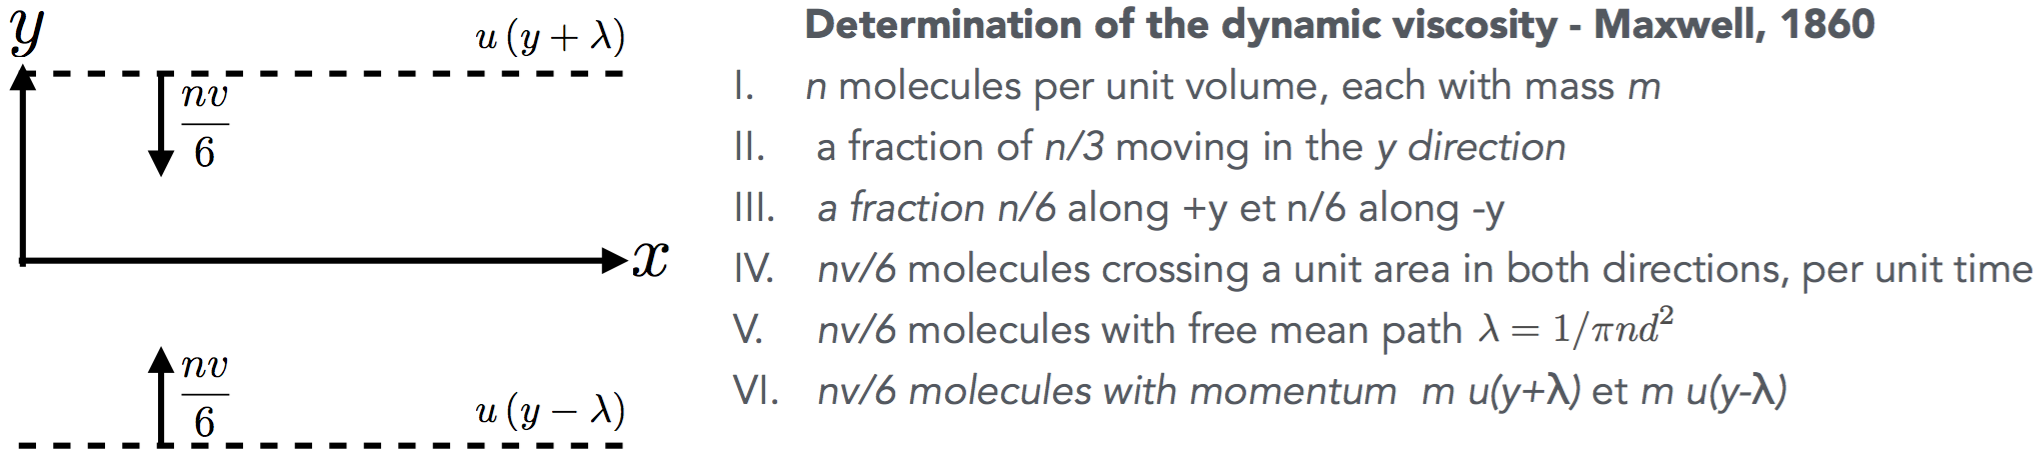
\includegraphics[scale=0.45]{ch1/8}
\end{center}
	
Let's consider a gas moving in the x direction with a velocity $u=u(y)$. The \textbf{kinetic theory} gives us the random velocity in $y$ using $v = \sqrt{\frac{3k_bT}{m}}$. The development of Maxwell, above, allows us to calculate the momentum flux crossing the x axis. $\frac{nv}{6}$ gives us the flux of particles for the y direction. 
\begin{equation}
	J_{Q_d} = \left(\frac{nv}{6}\right)mu(y-\lambda) - \left(\frac{nv}{6}\right)mu(y+\lambda)
\end{equation}
Here we use $u(y-\lambda)$ and $u(y+\lambda)$ because the last particles that can cross an axis on y are those who are situated in a distance of maximum $\lambda$ from there. \\
The Taylor expansion of the flux $u(y + \lambda) = u(\lambda) + \lambda\frac{du}{dy} + \dots$ and the constitutive equation \eqref{equation:1.11} gives us the final expression of viscosity 
\begin{equation}
	\mu = \frac{1}{3}nm\lambda v = \frac{1}{3}\rho \lambda v = \frac{1}{\pi \sqrt{3}}\frac{\sqrt{mk_bT}}{d^2}
	\label{equation:1.15}
\end{equation}
	
\subsection{Free mean path}
\begin{center}
	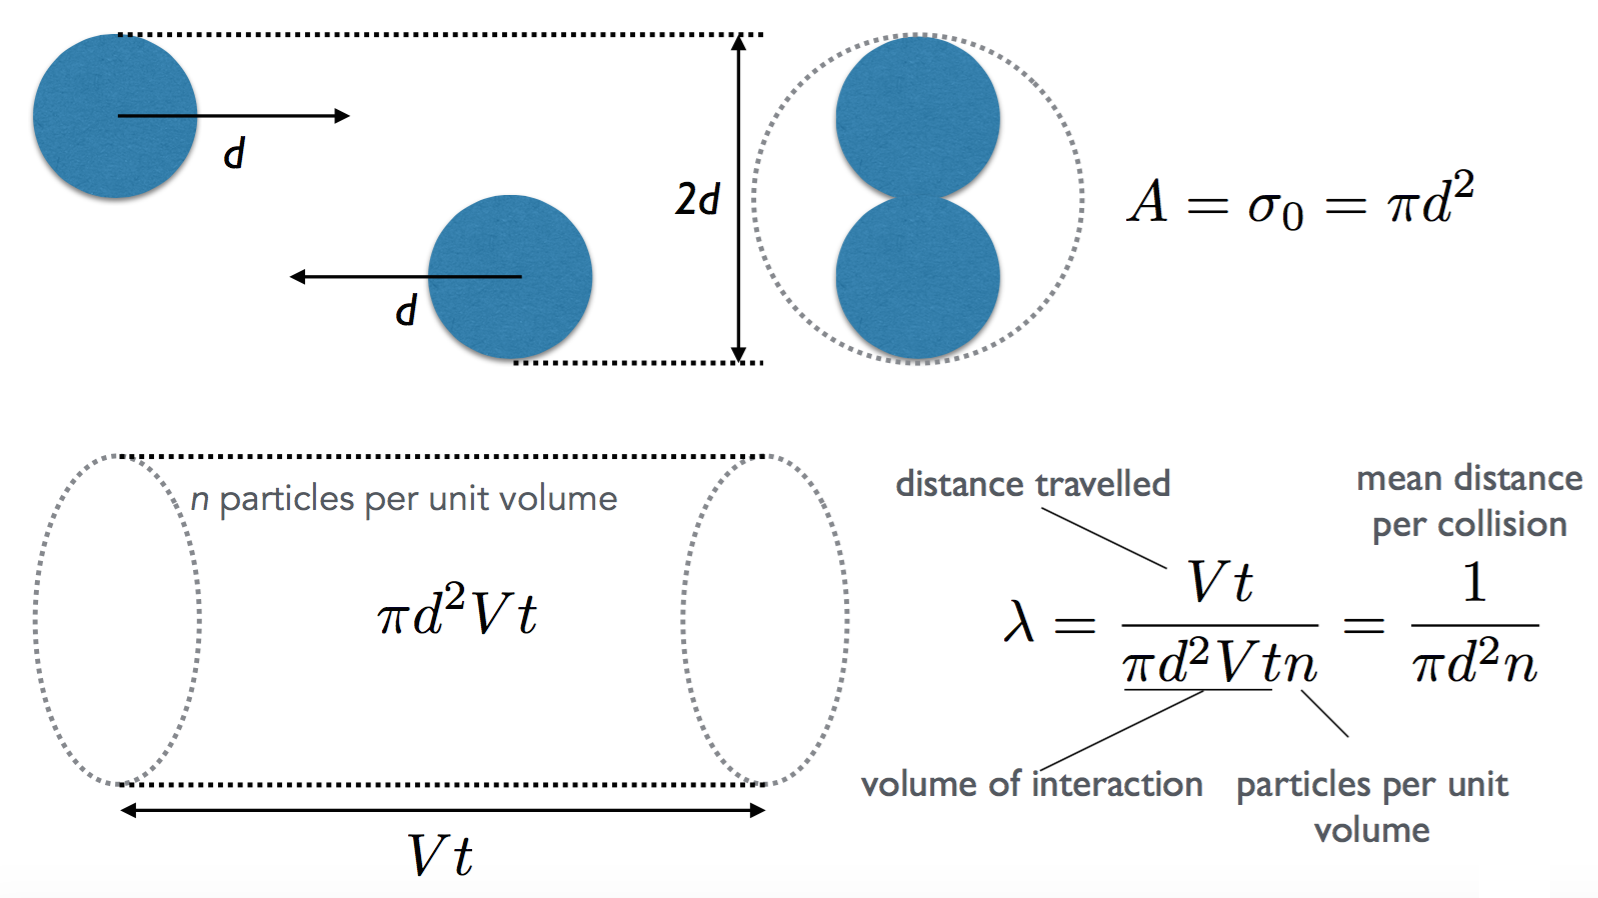
\includegraphics[scale=0.45]{ch1/9}
\end{center}
The slide above summarises the way to calculate the free mean path that is the average distance travelled by a particle between 2 collisions. First of all, we have to define a section of interaction. It's given by a circle of radius $d$. We also have to define a volume within the particles move. It's the cylinder of section $A$ and length $Vt$. The calculus of $\lambda$ is given by the distance travelled (without collision) divided by the volume where you can have interactions and by the particles per unit volume. 
	
\subsection{Viscosity variation with temperature}
\label{subsec:viscogas}
\begin{wrapfigure}[9]{r}{3.2cm}
	\vspace{-10mm}
	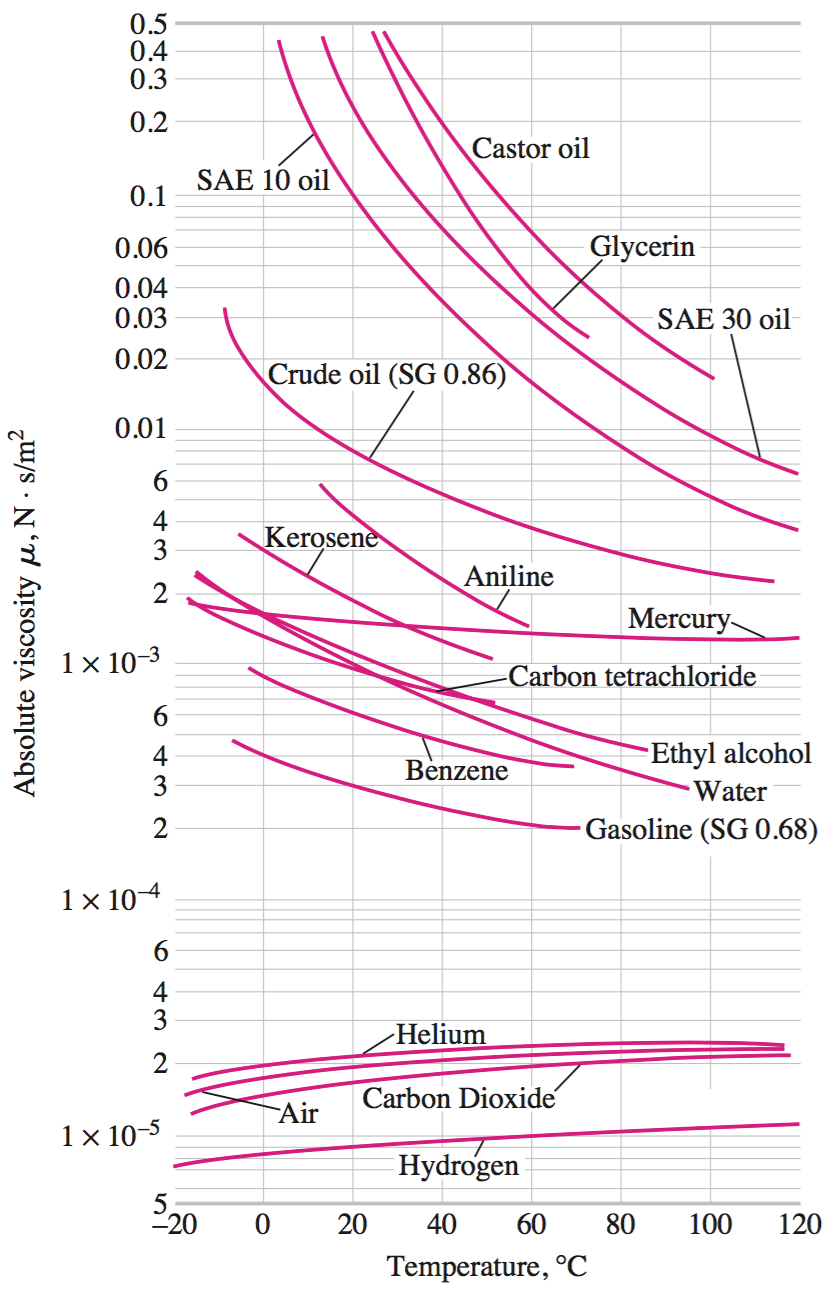
\includegraphics[scale=0.25]{ch1/10}
\end{wrapfigure}
We have said that gases viscosity increased with temperature. It's due to the kinetic approach that gave us the equation \eqref{equation:1.15} where $\mu \propto \sqrt{T}$. \\
For gases, the intermolecular forces are negligible. The increase in temperature makes particles move randomly at higher velocities conducting to more collisions per unit volume per unit time and so more resistance to flow. \\
For liquids, the increase in temperature decreases the viscosity because particles have higher energies that help them to oppose to the large cohesive intermolecular forces more strongly. They can thus move more freely. 

\subsection{Viscosity measurements}
	\begin{wrapfigure}[7]{l}{3.2cm}
	\vspace{-5mm}
	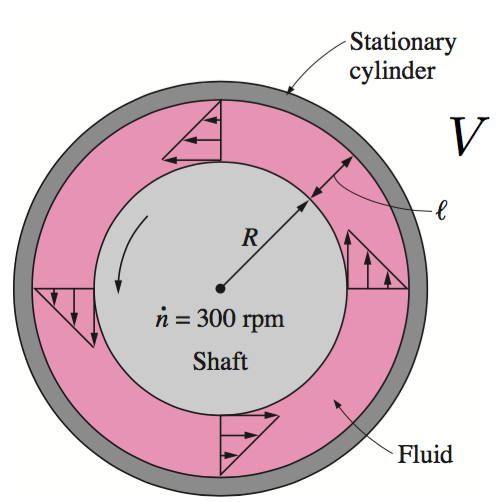
\includegraphics[scale=0.35]{ch1/16}
	\end{wrapfigure}
	Here is the principle of the viscometers composed of two concentric cylinders modelled as two flat plates separated by a fluid. Viscosity derived by torque, according to the figure we have
	\begin{equation}
		T = FR = \mu \frac{dv}{dr} A R = \frac{\mu 4 \pi ^2 R^3 rpmL}{l}
	\end{equation}
	where $A = 2\pi RL$ and $v = \omega R = 2\pi R rpm$
	
\subsection{Thermal conductivity}
\begin{center}
	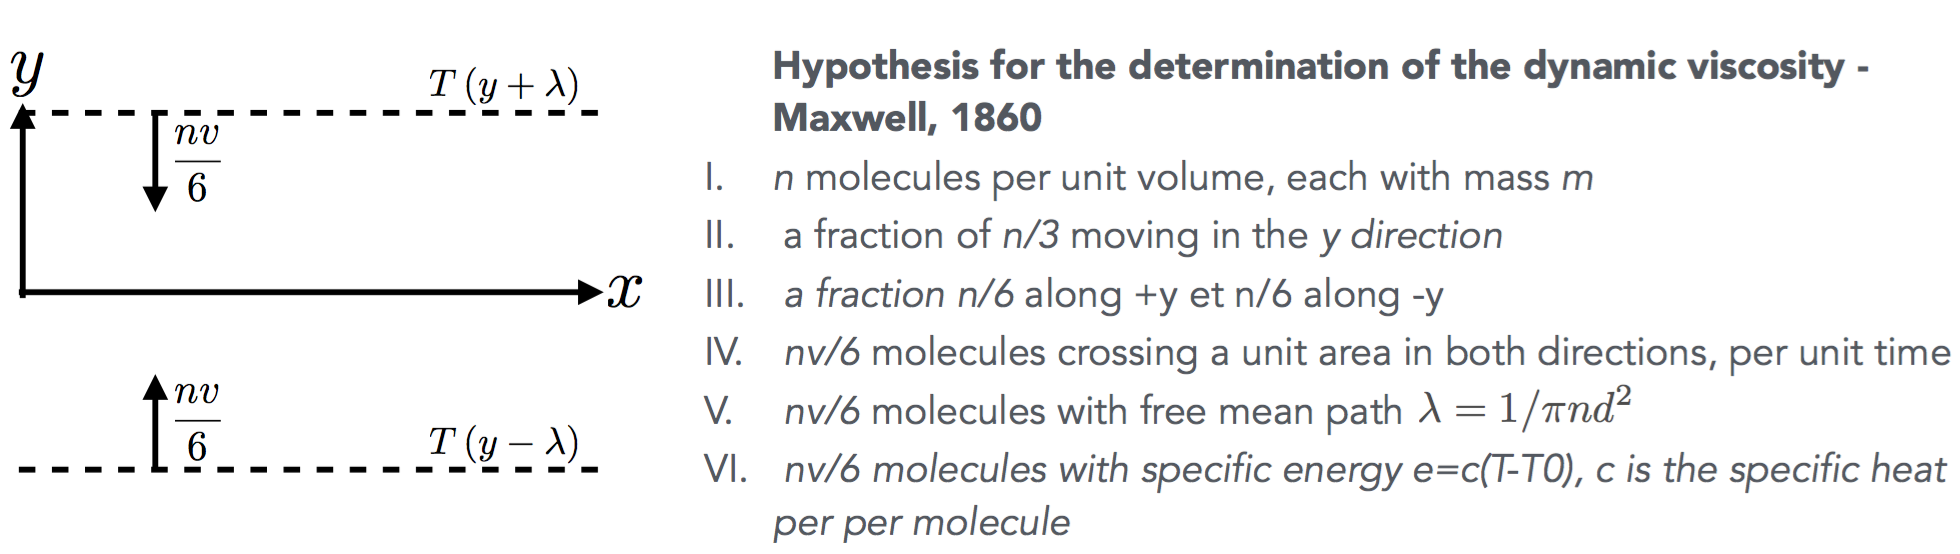
\includegraphics[scale=0.45]{ch1/17}
\end{center}
Similarly to the beginning of the section, let's consider a gas moving in the x direction with temperature $T=T(y)$. The velocity in y direction is random $v = \sqrt{\frac{3k_bT}{m}}$. The development presented above allows to calculate the diffusion flux 
\begin{equation}
	J_{ed} = \left(\frac{nv}{6} \right) [e(y-\lambda)] - \left(\frac{nv}{6} \right) [e(y+\lambda)]
\end{equation}
The constitutive equation being $J_{ed} = -k\frac{dT}{dy}$, we have
\begin{equation}
	k = \frac{1}{3} cn\lambda v = \frac{1}{\pi \sqrt{3}}\frac{c}{d^2}\sqrt{\frac{k_bT}{m}}
\end{equation}

\subsection{Mass diffusivity}
\begin{center}
	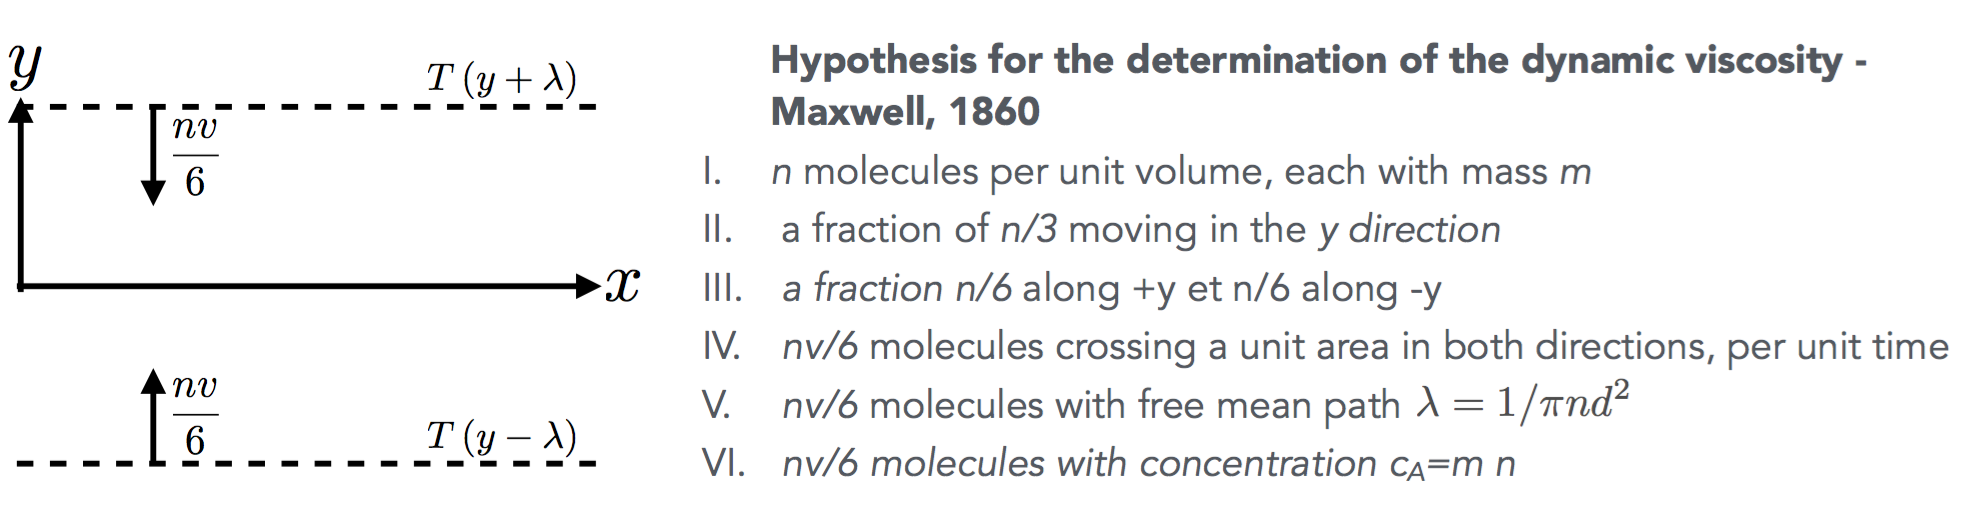
\includegraphics[scale=0.45]{ch1/18}
\end{center}
Same is done for mass diffusivity for a gas moving in the x direction with concentration  $C_A=C_A(y)$. The velocity in y direction is random $v = \sqrt{\frac{3k_bT}{m}}$. The development presented above allows to calculate the diffusion flux 
\begin{equation}
	J_{ad} = \left(\frac{nv}{6} \right) [n(y-\lambda)] - \left(\frac{nv}{6} \right) [n(y+\lambda)]
\end{equation}
The constitutive equation being $J_{ad} = -D\frac{dC_A}{dy}$, we have
\begin{equation}
	k = \frac{1}{3} \lambda v = \frac{1}{\pi \sqrt{3}}\frac{1}{nd^2}\sqrt{\frac{k_bT}{m}}
\end{equation}
Slide 33 can be read but it's too ugly to be asked in exam.

\section{Potential flow and boundary layer}
\subsection{Main aspects}
\begin{itemize}
	\item[•] The behaviour of a moving fluid element strongly depends on the \textbf{interactions} between the \textbf{fluid elements} and the \textbf{walls} for both internal and external flows. \\
	      	
	\item[•] Far from the walls, the shear stress and the dissipative forces are negligible. The fluid behaves \textbf{ideally}, is \textbf{incompressible} and \textbf{non-dissipative}. It's called a \textbf{potential} flow. \\
	      	
	\item[•] Potential flow are fully described by \textbf{Newtonian mechanics}, using the \textbf{conservation laws} for mass and mechanical energy, without any \textbf{dissipation} of mechanical \textbf{energy into heat}. \\
	      	
	\item[•] Close to the walls, the fluid velocity is \textbf{suddenly modified}, thus introducing \textbf{dissipative phenomena} that cannot be described using the potential flow theory.
	      	
	\item[•] The fluid layer thickness\footnote{Epaisseur} affected by the wall is named \textbf{boundary layer}\footnote{Couche limite} (as introduced by Prandtl, 1904).\\
	      	
	\item[•] Within the boundary layer, the velocity gradients in the flow normal direction as well as the shear stress in the direction parallel to the flow become extremely important.
\end{itemize}
	
\newpage
	
\subsection{Representation of the boundary layer}
\begin{wrapfigure}[6]{l}{4cm}
	\vspace{-5mm}
	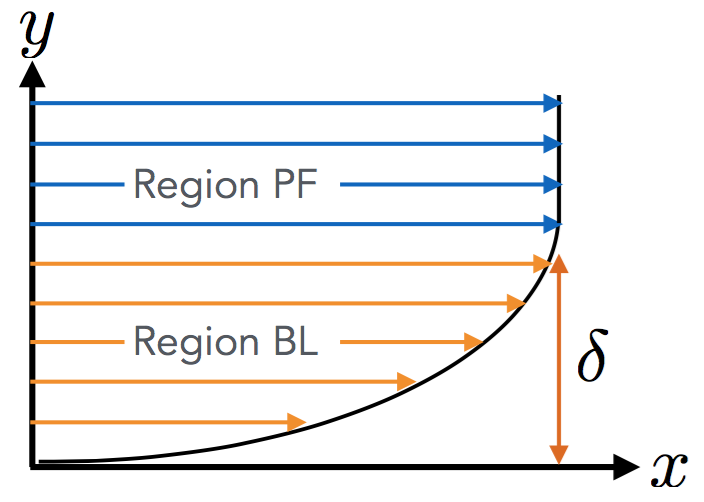
\includegraphics[scale=0.3]{ch1/11}
\end{wrapfigure}
We have to delimit two regions. The one (PF) within we have the \textbf{potential flow} that conserve his kinetic and potential energy (no dissipation) and the other (BL) within we have the \textbf{boundary layer} of thickness $\delta$, a velocity gradient with shear stress and dissipation of mechanical energy into heat. In the BL region appear two forces, a \textbf{drag} force that is due to friction, parallel to the flow and \textbf{lift} force that is a resistance perpendicular to the flow.  \\
In order to characterize the flow, we introduce the \textbf{Reynolds number}\\
\begin{equation}
	Re = \frac{\mbox{Convection}}{\mbox{Diffusion}} = \frac{J_{Q_c}}{J_{Q_d}} = \frac{\rho v^2}{\mu \frac{v}{L}} = \frac{vL}{\nu}
\end{equation}
that compares the convective and diffusive effect of the fluid momentum and the \textbf{Peclet number}
\begin{equation}
	P_{e_t} = \frac{J_{E_c}}{J_{E_d}} = \frac{\rho c_v v (T- T_0)}{k\frac{T}{L}} = \frac{vL}{\alpha} 
	\qquad and \qquad 
	P_{e_m} = \frac{J_{M_c}}{J_{M_d}} = \frac{vL}{D} 	
\end{equation}
that compares the convective and diffusive effect of the fluid energy and mass. Let's specify that if a uniform fluid flows towards a plate, we will have an \textbf{inviscid} flow region away from the plate and a \textbf{viscous} flow region next to the plate.
	
\subsection{Flow classification and friction force}
The classification is based on the Reynolds number. We have two types of fluid : \\
	
\begin{itemize}
	\item[•] $\mathbf{Re \gg 1 \rightarrow}$ \textbf{turbulent flow}, convection $>$ diffusion. \\
	      In that case, the fluid resistance (drag force) is independent of the viscosity and proportional to the momentum flux 
	      \begin{equation}
	      	F \approx \rho v^2 S
	      \end{equation}
	      
	\item[•] $\mathbf{Re \ll 1 \rightarrow}$ \textbf{laminar flow}, convection $<$ diffusion. \\
	      In that case, the fluid resistance is function of the viscosity and proportional to the diffusive momentum flux
	      \begin{equation}
	      	F \approx \mu L v
	      \end{equation}
\end{itemize}
	
\subsection{Determination of the boundary layer thickness}
The separation between the two regimes above is not possible. Consider a wind flow around a building. The Reynolds number will be high meaning the flow is turbulent. Indeed, the \textbf{approaching flow} can be classified as a potential flow, whereas \textbf{close to the walls} the dissipative effects will take place with the conversion of mechanical energy into heat. \\
So, far from the walls the dominant transport mechanism will be convection and close to the walls viscous transport. At a distance equal to the boundary layer thickness, \textbf{convection and diffusion will be comparable}. This allows us determining its \textbf{order of magnitude}.
	
\begin{center}
	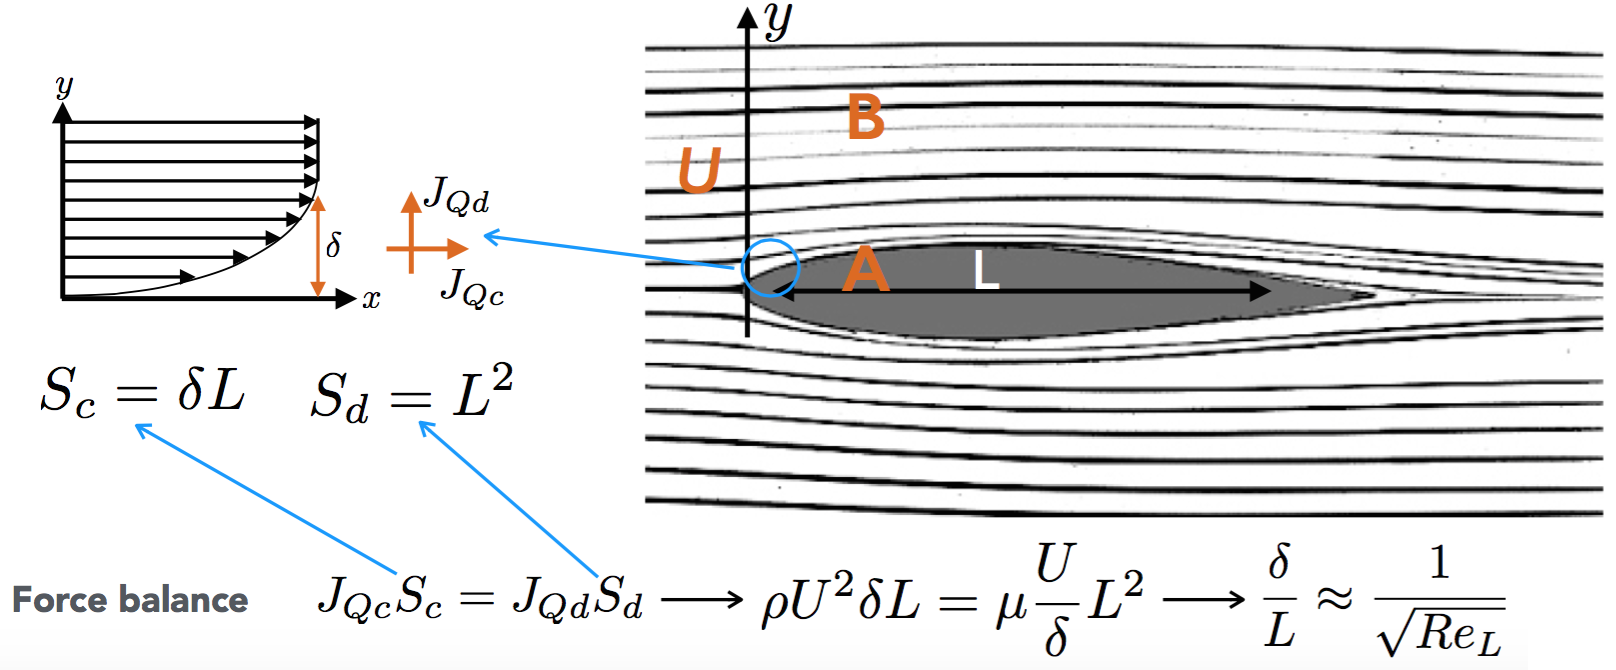
\includegraphics[scale=0.4]{ch1/12}
\end{center}
We can qualitatively find $\delta$ as the distance from the wall at which the convective momentum flux (\textbf{parallel} to the flow) equals the diffusive one (\textbf{perpendicular} to the flow). For that, let's take a section in which convection dominates ($S_c$) and another in which diffusion dominates ($S_d$). When we equalize the two flux expressed respectively for convection and diffusion, we arrive to the magnitude of $\delta$ compared to $L$.
	
\subsection{Features of the boundary layer and practical consequences}
The relative dimension of the boundary layer is inversely proportional to $Re^{0.5}$ and the absolute dimension is proportional to $L^{0.5}$.

\subsubsection{Consequences for internal flows}
\begin{wrapfigure}[5]{r}{4cm}
	\vspace{-5mm}
	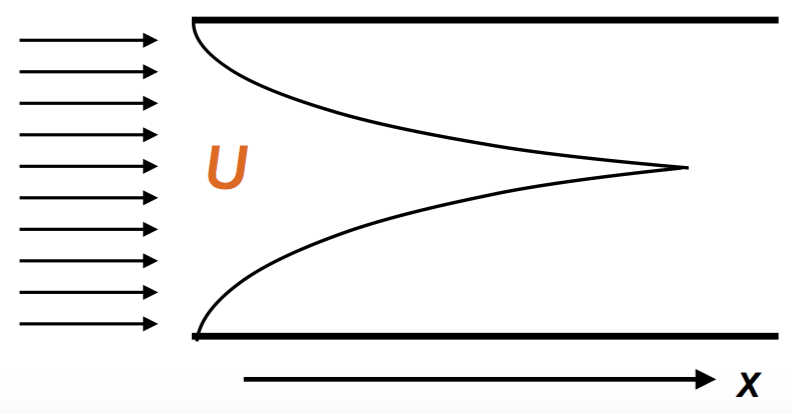
\includegraphics[scale=0.3]{ch1/13}
\end{wrapfigure}
The boundary layer thickness increases with $x^{0.5}$ and far from the inlet\footnote{La prise - l'entrée}, the boundary layer will extend to the full diameter pipe. 
\begin{equation}
	\frac{\delta}{x} \approx \frac{1}{\sqrt{Re_x}} \qquad and \qquad \delta \approx \sqrt{\frac{xv}{U}}
\end{equation}
	
\subsubsection{Consequences for external flows}
\begin{wrapfigure}[5]{l}{5cm}
	\vspace{-5mm}
	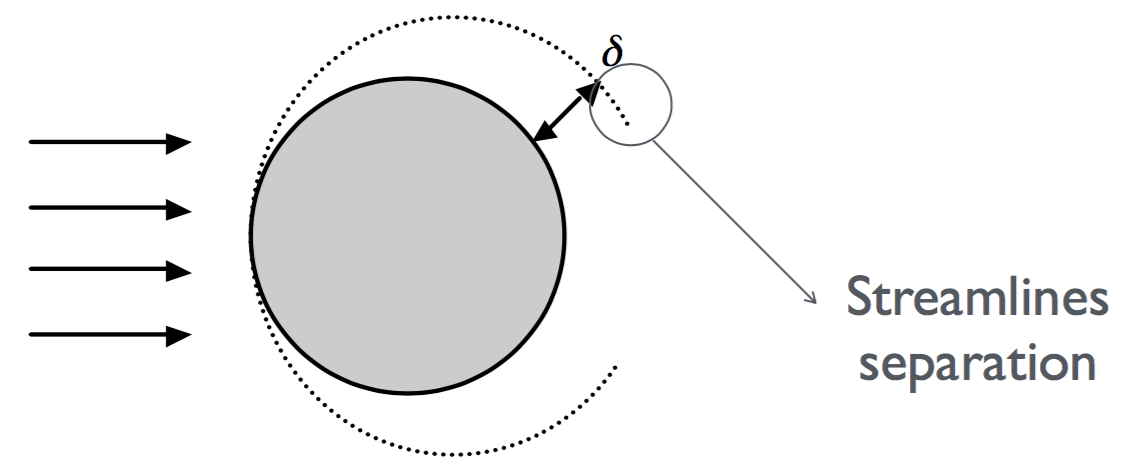
\includegraphics[scale=0.25]{ch1/14}
\end{wrapfigure}	
The boundary layer cannot infinitely grow. It will be thinner in front the body and thicker behind it. Behind the body, the flow streamlines detach. If the boundary layer thickness is known, the force exerted by the flow can be directly evaluated, being the velocity gradient of the order $\frac{U}{\delta}$, which gives a shear stress of $\tau = \mu\frac{U}{\delta}$ on the walls. The drag force will be then higher in front of the body (where the boundary layer is thinner) and lower behind it (where the boundary layer is thicker). From symmetry considerations, the drag force only acts in the flow direction. \\
More commonly, a perpendicular component also exists called \textbf{lift} but here it doesn't appear. 
	
\begin{equation}
	F = \int _S \mu \frac{dv}{dy} \, dS
\end{equation}
	
\begin{wrapfigure}[6]{r}{6cm}
	\vspace{-5mm}
	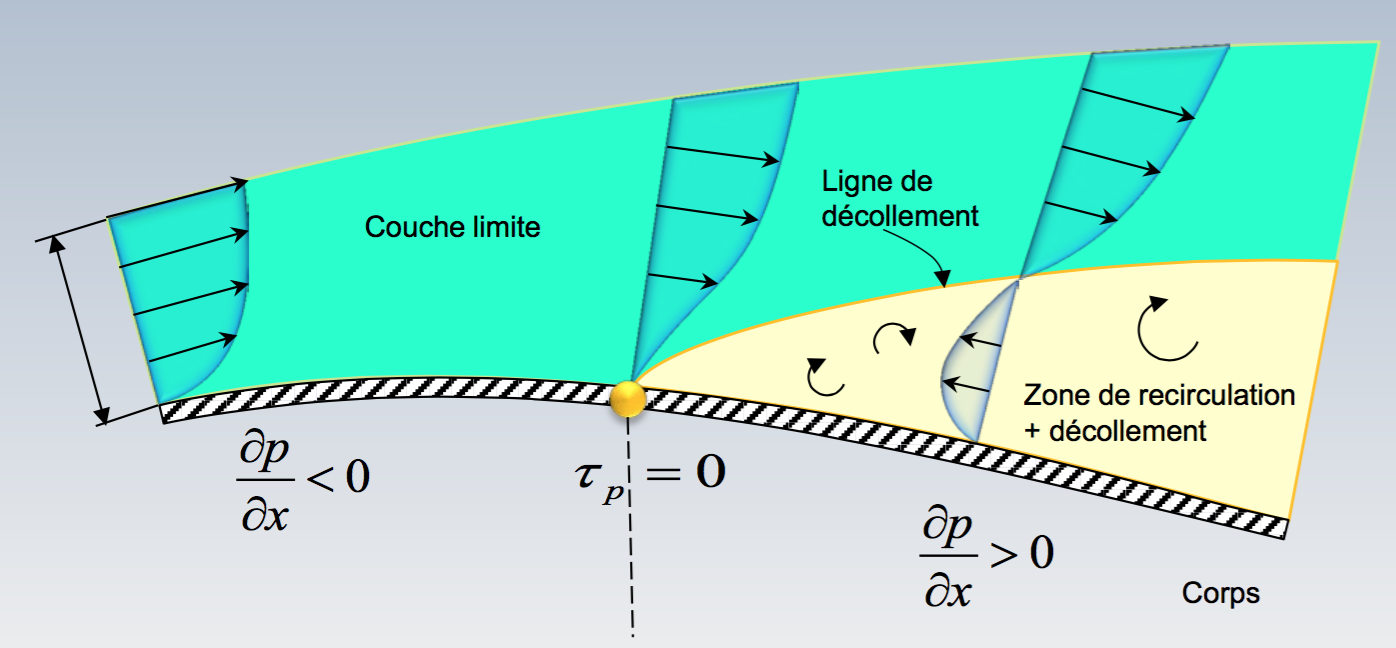
\includegraphics[scale=0.25]{ch1/15}
\end{wrapfigure}
Here's an illustration of the flow separation. There is a \textbf{recirculation} region which provides a force opposed to the flow. In order to maximise the body speed, it is necessary to reduce the drag force due to the flow separation.  